%%%%%%%%%%%%%%%%%%%%%%%%%%%%%%%%%%%%%
%                                   %
% Compile with XeLaTeX and biber    %
%                                   %
% Questions or comments:            %
%                                   %
% joshua dot mcneill at uga dot edu %
%                                   %
%%%%%%%%%%%%%%%%%%%%%%%%%%%%%%%%%%%%%

\documentclass{beamer}
  % Read in standard preamble (cosmetic stuff)
  %%%%%%%%%%%%%%%%%%%%%%%%%%%%%%%%%%%%%%%%%%%%%%%%%%%%%%%%%%%%%%%%
% This is a standard preamble used in for all slide documents. %
% It basically contains cosmetic settings.                     %
%                                                              %
% Joshua McNeill                                               %
% joshua dot mcneill at uga dot edu                            %
%%%%%%%%%%%%%%%%%%%%%%%%%%%%%%%%%%%%%%%%%%%%%%%%%%%%%%%%%%%%%%%%

% Beamer settings
% \usetheme{Berkeley}
\usetheme{CambridgeUS}
% \usecolortheme{dove}
% \usecolortheme{rose}
\usecolortheme{seagull}
\usefonttheme{professionalfonts}
\usefonttheme{serif}
\setbeamertemplate{bibliography item}{}

% Packages and settings
\usepackage{fontspec}
  \setmainfont{Charis SIL}
\usepackage{hyperref}
  \hypersetup{colorlinks=true,
              allcolors=blue}
\usepackage{graphicx}
  \graphicspath{{../../figures/}}
\usepackage[normalem]{ulem}
\usepackage{enumerate}

% Document information
\author{M. McNeill}
\title[FREN2001]{Français 2001}
\institute{\url{joshua.mcneill@uga.edu}}
\date{}

%% Custom commands
% Lexical items
\newcommand{\lexi}[1]{\textit{#1}}
% Gloss
\newcommand{\gloss}[1]{`#1'}
\newcommand{\tinygloss}[1]{{\tiny`#1'}}
% Orthographic representations
\newcommand{\orth}[1]{$\langle$#1$\rangle$}
% Utterances (pragmatics)
\newcommand{\uttr}[1]{`#1'}
% Sentences (pragmatics)
\newcommand{\sent}[1]{\textit{#1}}
% Base dir for definitions
\newcommand{\defs}{../definitions}


  % Packages and settings
  \usepackage[backend=biber, style=apa]{biblatex}
    \addbibresource{../references/References.bib}
  \usepackage[linguistics]{forest}

  % Document information
  \subtitle[Constructing a Grammar]{Constructing a Grammar}

  %% Custom commands
  % Subsection/frame titles
  \newcommand{\suboneone}{What's this about?}
  \newcommand{\subonetwo}{The elements}
  \newcommand{\subonethree}{The rules}
  \newcommand{\subonefour}{Ambiguity}
  \newcommand{\subonefive}{A warning}
  \newcommand{\subonesix}{Resources and practice}

\begin{document}
  % Read in the standard intro slides (title page and table of contents)
  %%%%%%%%%%%%%%%%%%%%%%%%%%%%%%%%%%%%%%%%%%%%%%%%%%%%%%%%%%%%%%%%
% This is a standard set of intro slides used in for all slide %
% documents. It basically contains the title page and table of %
% contents.                                                    %
%                                                              %
% Joshua McNeill                                               %
% joshua dot mcneill at uga dot edu                            %
%%%%%%%%%%%%%%%%%%%%%%%%%%%%%%%%%%%%%%%%%%%%%%%%%%%%%%%%%%%%%%%%

\begin{frame}
  \titlepage
  \tiny{Office: % Basically a variable for office hours location
Gilbert 121\\
        Office hours: % Basically a variable for office hours
 lundi, mercredi, vendredi 10:10--11:10
}
\end{frame}

\begin{frame}
  \tableofcontents[hideallsubsections]
\end{frame}

\AtBeginSection[]{
  \begin{frame}
    \tableofcontents[currentsection,
                     hideallsubsections]
  \end{frame}
}


  \section{Constructing a grammar}
    \subsection{\suboneone}
      \begin{frame}[t]{\suboneone}
        \begin{block}{}
          Constructing a grammar is equivalent to making a claim about how some speaker's language is organized in their mind
        \end{block}
        \only<2>{
          \begin{columns}
            \column{0.5\linewidth}
              \begin{block}{Useful for}
                The sake of knowledge
              \end{block}
            \column{0.5\linewidth}
              
\includegraphics[scale=0.15]{knowledge.jpg}
          \end{columns}
        }
        \only<3>{
          \begin{block}{Useful for}
            Language learners
          \end{block}
          \begin{center}
            
\includegraphics[scale=0.085]{lang_learning.jpg}
          \end{center}
        }
        \only<4>{
          \begin{block}{Useful for}
            Computational systems
          \end{block}
          \begin{center}
            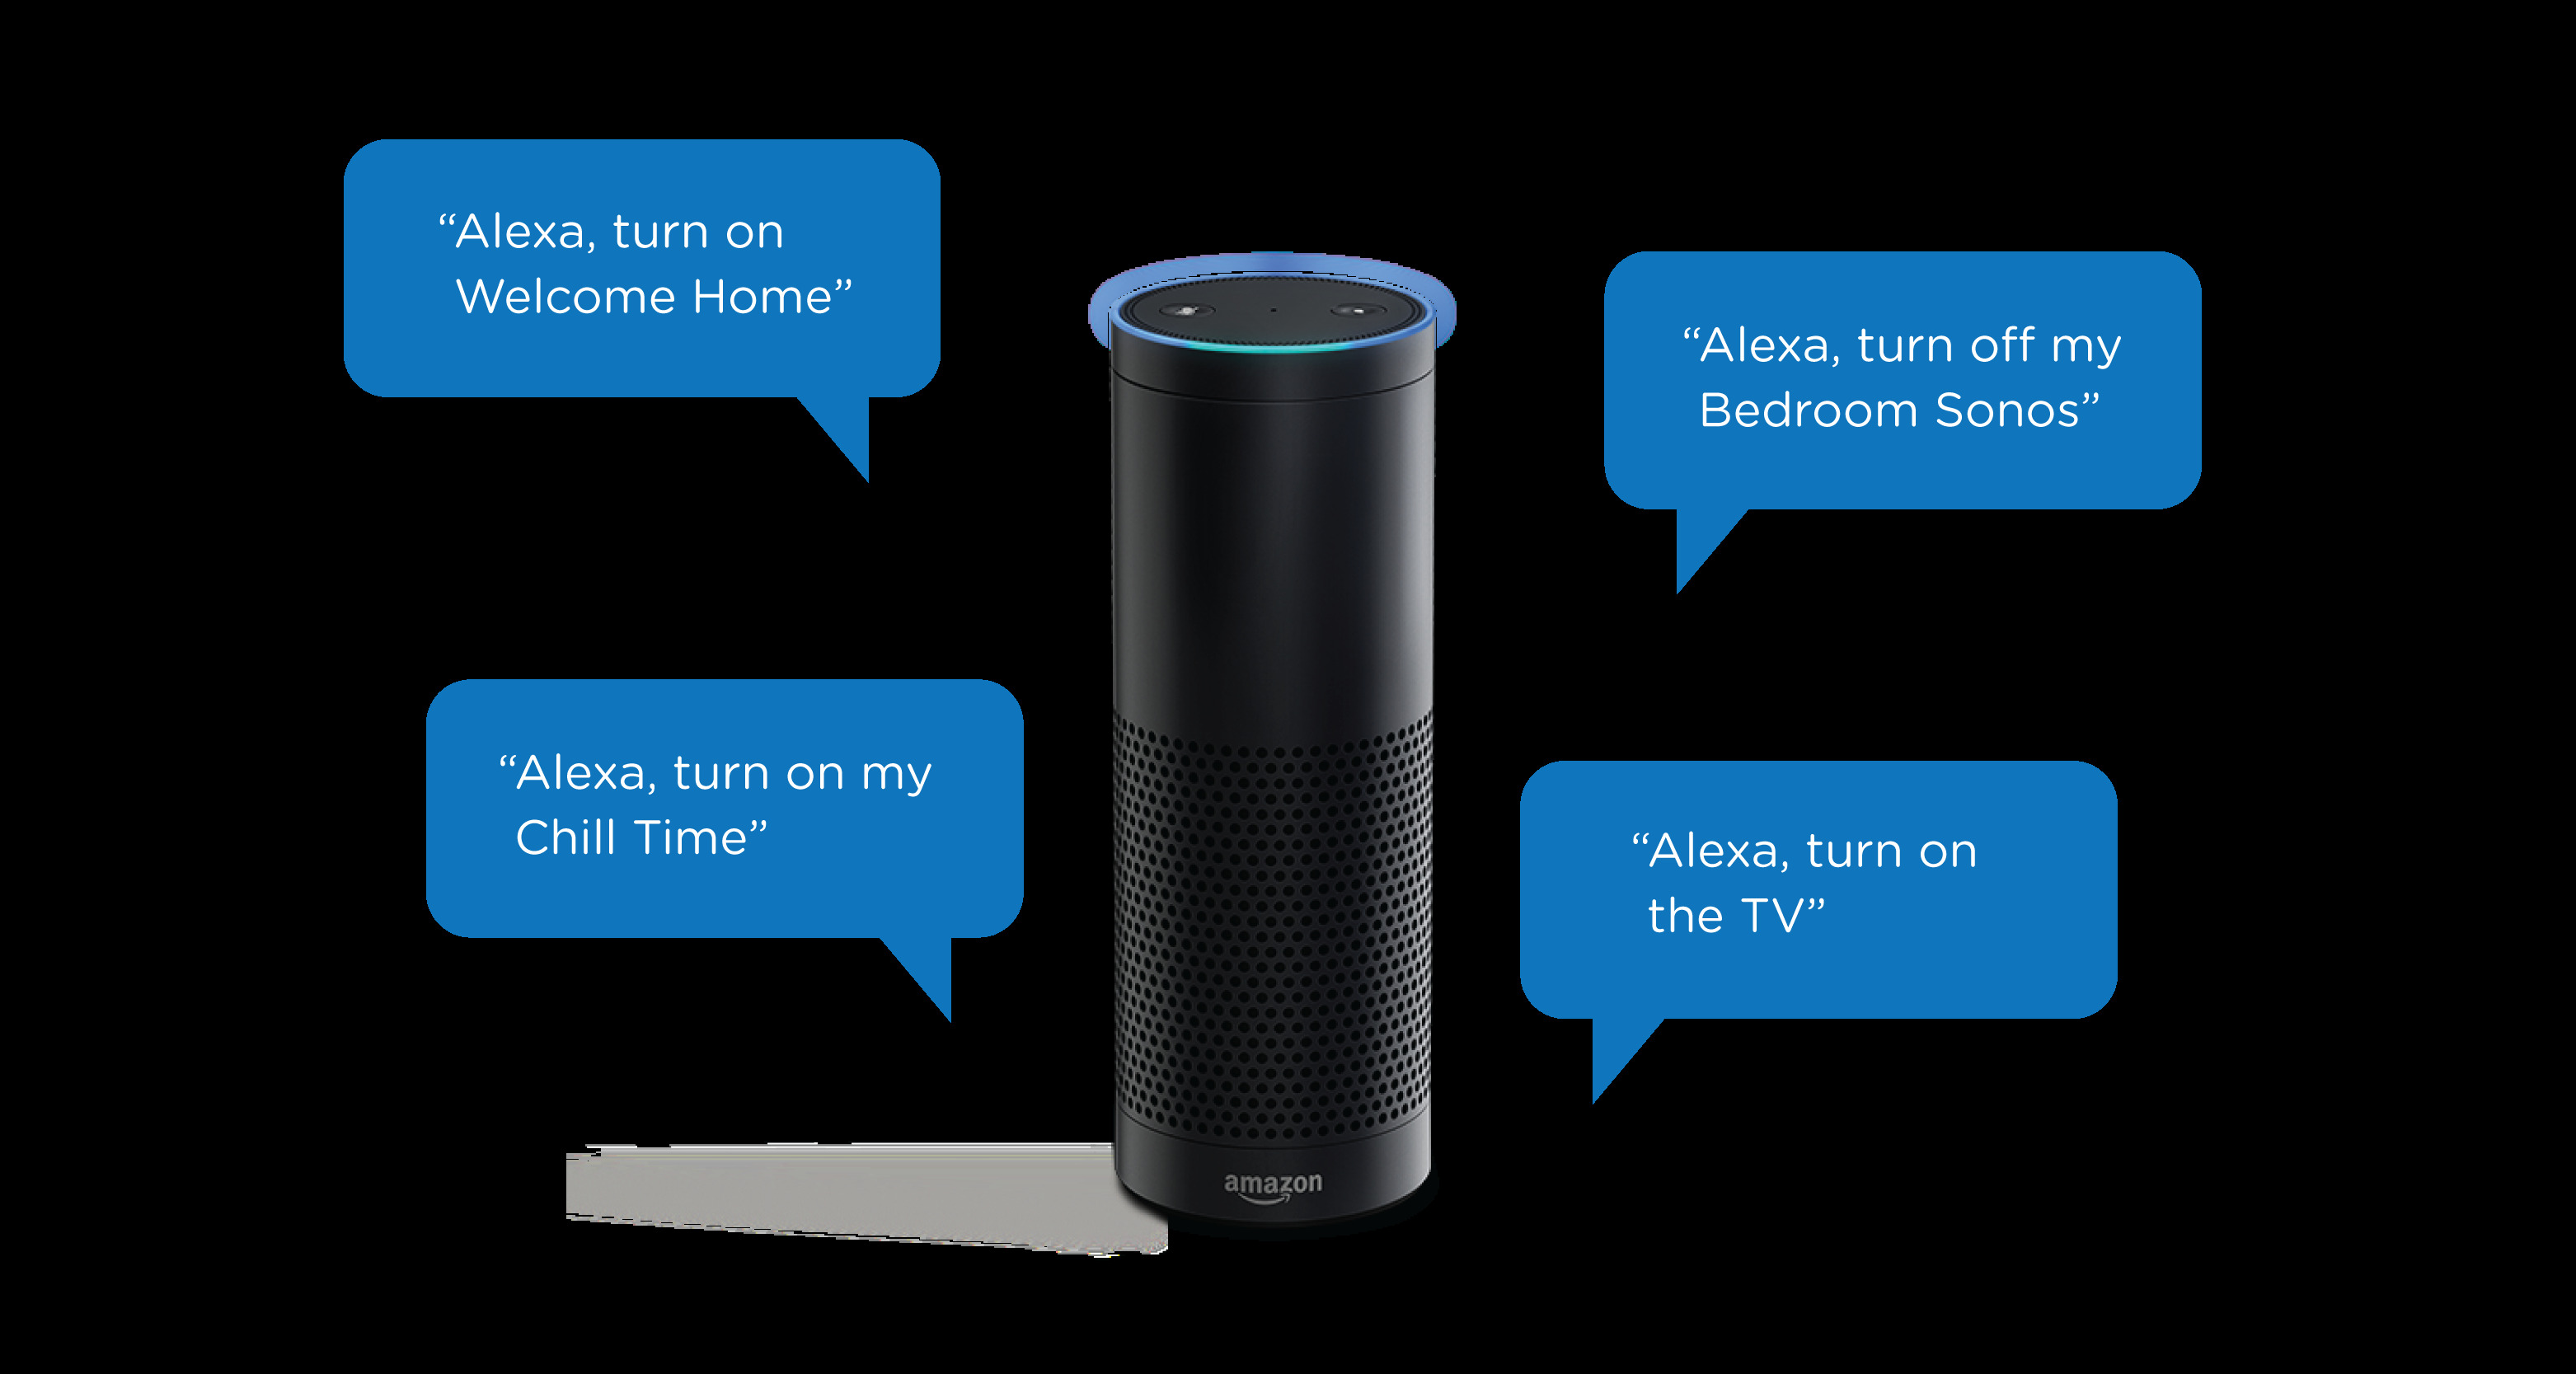
\includegraphics[scale=0.105]{alexa.jpg}
          \end{center}
        }
        \only<5>{
          \begin{block}{Our goal}
            Construct a grammar for English syntax using what we've learned about syntax so far
          \end{block}
        }
      \end{frame}

    \subsection{\subonetwo}
      \begin{frame}[t]{\subonetwo}
        \begin{block}{Four types of elements involved}
          \begin{itemize}
            \item Broad constituents
            \item Syntactic categories
            \item Lexical categories
            \item Lexical expressions
          \end{itemize}
        \end{block}
        \only<2>{
          \begin{block}{Broad constituents (not a technical term)}
            For now,
            \begin{itemize}
              \item S: Sentence
            \end{itemize}
          \end{block}
        }
        \only<3-4>{
          \begin{block}{Syntactic categories}
            \uncover<4->{
              % Syntactic category
A group to which expressions that share the same syntactic distribution and syntactic properties belong

              \begin{itemize}
                \item e.g., NP, VP, AP, and PP
              \end{itemize}
            }
          \end{block}
        }
        \only<5-6>{
          \begin{block}{Lexical categories}
            \uncover<6->{
              % Lexical category
A word's classification based on its behavior in sentences and some general aspects of its meaning (e.g., noun, verb, adjective)

              \begin{itemize}
                \item e.g., Det, N, V, Adj, P, and Adv
              \end{itemize}
            }
          \end{block}
        }
        \only<7-8>{
          \begin{block}{Lexical expressions}
            \uncover<8->{
              % Lexical expression
A linguistic expression that is part of one's mental lexicon

              \begin{itemize}
                \item e.g., the, dog, eat, small, with, very, etc.
              \end{itemize}
            }
          \end{block}
        }
      \end{frame}

    \subsection{\subonethree}
      \begin{frame}[t]{\subonethree}
        \begin{alertblock}{Phrase structure rewrite rules \parencite{chomsky_syntactic_2002}}
          % Phrase structure rewrite rule
An operation which converts a constituent or lexical category into its part(s)

        \end{alertblock}
        \only<2-4>{
          \begin{block}{The rule for S}
            S $\rightarrow$ NP VP
          \end{block}
          \only<2-3>{
            \begin{example}
              S $\rightarrow$ [NP the very green cat] [VP eats the mouse in the alley]
            \end{example}
            \begin{block}<3->{Usually not VP NP unless you're Yoda}
              S $\rightarrow$ [VP eats the mouse in the alley] [NP the very green cat]
            \end{block}
          }
          \only<4>{
            \begin{block}{}
              NP and VP are immediate constituents of S
            \end{block}
            \begin{alertblock}{Immediate constituents}
              % Immediate constituents
The elements into which a higher level element is broken down through a single phrase structure rewrite rule

            \end{alertblock}
          }
        }
      \end{frame}

      \begin{frame}{\subonethree}
        \begin{block}{}
          We can diagram S $\rightarrow$ NP VP as a \alert{phrase structure tree}:
          \begin{itemize}
            \item % Phrase structure tree
A visual representation of the structure of a sentence

          \end{itemize}
        \end{block}
        \begin{forest}
          [S
            [NP
              [the very green cat]
            ]
            [VP
              [eats the mouse in the alley]
            ]
          ]
        \end{forest}
      \end{frame}

      \begin{frame}[t]{\subonethree}
        \begin{block}{The rule for NP}
          NP $\rightarrow$ Det N
        \end{block}
        \begin{forest}
          [S
            [NP
              [the very green cat]
            ]
            [VP
              [eats]
              [NP
                [D
                  [the]
                ]
                [N
                  [mouse]
                ]
              ]
              [in the alley]
            ]
          ]
        \end{forest}
      \end{frame}

      \begin{frame}[t]{\subonethree}
        \begin{block}{The more extensive rule for NP}
          NP $\rightarrow$ (Det) (AP)* N (PP)*
        \end{block}
        \begin{forest}
          [S
            [NP
              [Det
                [the]
              ]
              [AP
                [very green]
              ]
              [N
                [cat]
              ]
            ]
            [VP
              [eats]
              [NP
                [D
                  [the]
                ]
                [N
                  [mouse]
                ]
              ]
              [in the alley]
            ]
          ]
        \end{forest}
      \end{frame}

      \begin{frame}[t]{\subonethree}
        \begin{block}{The rule for VP}
          VP $\rightarrow$ V (NP)* (AP) (PP)*
        \end{block}
        \begin{forest}
          [S
            [NP
              [Det
                [the]
              ]
              [AP
                [very green]
              ]
              [N
                [cat]
              ]
            ]
            [VP
              [V
                [eats]
              ]
              [NP
                [D
                  [the]
                ]
                [N
                  [mouse]
                ]
              ]
              [PP
                [in the alley]
              ]
            ]
          ]
        \end{forest}
      \end{frame}

      \begin{frame}[t]{\subonethree}
        \begin{block}{The rule for PP}
          PP $\rightarrow$ P NP
        \end{block}
        \small
        \begin{forest}
          [S
            [NP
              [Det
                [the]
              ]
              [AP
                [very green]
              ]
              [N
                [cat]
              ]
            ]
            [VP
              [V
                [eats]
              ]
              [NP
                [D
                  [the]
                ]
                [N
                  [mouse]
                ]
              ]
              [PP
                [P
                  [in]
                ]
                [NP
                  [Det
                    [the]
                  ]
                  [N
                    [alley]
                  ]
                ]
              ]
            ]
          ]
        \end{forest}
      \end{frame}

      \begin{frame}[t]{\subonethree}
        \begin{block}{The rule for AP}
          AP $\rightarrow$ (Adv)* Adj
        \end{block}
        \small
        \begin{forest}
          [S
            [NP
              [Det
                [the]
              ]
              [AP
                [Adv
                  [very]
                ]
                [Adj
                  [green]
                ]
              ]
              [N
                [cat]
              ]
            ]
            [VP
              [V
                [eats]
              ]
              [NP
                [D
                  [the]
                ]
                [N
                  [mouse]
                ]
              ]
              [PP
                [P
                  [in]
                ]
                [NP
                  [Det
                    [the]
                  ]
                  [N
                    [alley]
                  ]
                ]
              ]
            ]
          ]
        \end{forest}
      \end{frame}

      \begin{frame}{\subonethree}
        \begin{block}{}
          Our grammar of English syntax, then
        \end{block}
        \begin{block}{}
          \begin{itemize}
            \item S $\rightarrow$ NP VP
            \item NP $\rightarrow$ (Det) (AP)* N (PP)*
            \item VP $\rightarrow$ V (NP)* (AP) (PP)*
            \item PP $\rightarrow$ P NP
            \item AP $\rightarrow$ (Adv)* Adj
          \end{itemize}
        \end{block}
      \end{frame}

    \subsection{\subonefour}
      \begin{frame}{\subonefour}
        \begin{block}{Remember linguistics expressions}
          % Linguistic expression
A piece of language with a certain form, a certain meaning, and certain syntactic properties

        \end{block}
        \begin{alertblock}<2->{}
          \emph{But}, an expression can have one form and multiple unrelated meanings and syntactic properties
        \end{alertblock}
      \end{frame}

      \begin{frame}{\subonefour}
        \begin{example}
          \lexi{Bank}, whose form is [ˈbæŋk], has two unrelated meanings:
          \begin{itemize}
            \item<2-> Where you keep your money
            \begin{itemize}
              \item<2-> e.g., The bank\textsubscript{1} charges too many fees.
            \end{itemize}
            \item<2->  The edge of a body of water
            \begin{itemize}
              \item<2-> e.g., Along the bank\textsubscript{2} of the Oconee River is a nice place to walk.
            \end{itemize}
          \end{itemize}
        \end{example}
      \end{frame}

      \begin{frame}{\subonefour}
        \begin{alertblock}{Ambiguity}
          % Ambiguity
The phenomenon by which a linguistic expression has one form and multiple unrelated meanings or syntactic properties

        \end{alertblock}
        \begin{block}{Two types}
          \begin{itemize}
            \item Lexical ambiguity
            \item Structural ambiguity
          \end{itemize}
        \end{block}
      \end{frame}

      \begin{frame}[t]{\subonefour}
        \begin{alertblock}{Lexical ambiguity}
          % Lexical ambiguity
The phenomenon by which a lexical expression has one form and multiple unrelated meanings or syntactic properties

        \end{alertblock}
        \only<2>{
          \begin{block}{}
            It can be based on meaning
          \end{block}
          \begin{example}
            \lexi{Bank}\textsubscript{1} and \lexi{bank}\textsubscript{2} differed only in meaning
            \begin{itemize}
              \item The fee charging place is still a N
              \item The edge of the water is still a N
            \end{itemize}
          \end{example}
        }
        \only<3-4>{
          \begin{block}{}
            It can be based on syntactic properties
          \end{block}
          \begin{example}
            \lexi{Bank} has two unrelated lexical categories:
            \begin{itemize}
              \item<4-> N (e.g., The bank\textsubscript{1} charges too many fees.)
              \item<4-> V (e.g., You should bank\textsubscript{3} your money there anyway.)
            \end{itemize}
          \end{example}
        }
      \end{frame}

      \begin{frame}[t]{\subonefour}
        \begin{alertblock}{Structural ambiguity}
          % Structural ambiguity
The phenomenon by which a phrasal expression has one form and multiple unrelated meanings or syntactic properties

          \begin{itemize}
            \item In this case, we mean the form of S is the same
          \end{itemize}
        \end{alertblock}
        \begin{example}<2->
          These Ss have the same form but two interpretations
          \begin{enumerate}
            \item The green cat saw the alien with the telescope.
            \begin{itemize}
              \item<3-> `The green cat used a telescope to see the alien.'
            \end{itemize}
            \item The green cat saw the alien with the telescope.
            \begin{itemize}
              \item<3-> `The alien was holding a telescope when the green cat saw it.'
            \end{itemize}
          \end{enumerate}
        \end{example}
      \end{frame}

      \begin{frame}[t]{\subonefour}
        \begin{block}{Which interpretation is this?}
          \uncover<2->{`The alien was holding a telescope when the green cat saw it.'}
        \end{block}
        \tiny
        \begin{center}
          \begin{forest}
            [S
              [NP
                [Det
                  [The]
                ]
                [AP
                  [Adj
                    [green]
                  ]
                ]
                [N
                  [cat]
                ]
              ]
              [VP
                [V
                  [saw]
                ]
                [NP
                  [Det
                    [the]
                  ]
                  [N
                    [alien]
                  ]
                  [PP
                    [P
                      [with]
                    ]
                    [NP
                      [Det
                        [the]
                      ]
                      [N
                        [telescope]
                      ]
                    ]
                  ]
                ]
              ]
            ]
          \end{forest}
        \end{center}
      \end{frame}

      \begin{frame}[t]{\subonefour}
        \begin{block}{Which interpretation is this?}
          \uncover<2->{`The green cat used a telescope to see the alien.'}
        \end{block}
        \tiny
        \begin{center}
          \begin{forest}
            [S
              [NP
                [Det
                  [The]
                ]
                [AP
                  [Adj
                    [green]
                  ]
                ]
                [N
                  [cat]
                ]
              ]
              [VP
                [V
                  [saw]
                ]
                [NP
                  [Det
                    [the]
                  ]
                  [N
                    [alien]
                  ]
                ]
                [PP
                  [P
                    [with]
                  ]
                  [NP
                    [Det
                      [the]
                    ]
                    [N
                      [telescope]
                    ]
                  ]
                ]
              ]
            ]
          \end{forest}
        \end{center}
      \end{frame}

    \subsection{\subonefive}
      \begin{frame}{\subonefive}
        \begin{block}{Our grammar is pretty good, but}
          It doesn't generate all possible sentences:
          \begin{itemize}
            \item The green cat [that likes gumbo] saw the alien [who came in peace].
          \end{itemize}
        \end{block}
      \end{frame}

    \subsection{\subonesix}
      \begin{frame}{\subonesix}
        \begin{block}{}
          % A set of links to useful resources when working with syntax
\begin{itemize}
  \item To draw trees on a computer: \url{https://ironcreek.net/syntaxtree/}
\end{itemize}

        \end{block}
        \begin{block}{Try these}
          \textcite{dawson_language_2016}, chapter 5 exercise 27
        \end{block}
      \end{frame}

      \begin{frame}{References}
        \printbibliography
      \end{frame}
\end{document}
